%!TEX root = ../main.tex
\section{NGT--DAQ Integration} % Thiago

%%% We just write the discussion we had in the whole DAQ session

The Optimal Calibration system has to be embedded in the CMS trigger and data acquisition (DAQ) system,
both in the demonstrator system and in the Phase-2 implementation.
We briefly discuss the DAQ system architecture implemented for Run 3, 
and how the demonstrator can be inserted in that system.
We then review the conceptual DAQ design proposed for Phase-2, and 
go through a preliminary calculation of the NGT system feasibility.

\subsection{Demonstrator Integration in Run 3}

The CMS DAQ system for Run 3 (DAQ3) is an intricate system, dealing with all steps of the data flow from the sub-detector front-end drivers (FEDs) through the final delivery of data streams to Tier-0. For the purposes of our discussions, we can focus on the following elements of Figure~\ref{fig:DAQ3}: 
the \emph{Readout Units} (RUs) unpack and merge event fragments into super-fragments, which are then sent to the \emph{Builder Units} (BUs) to be further assembled into complete events. 
The complete events are sent to the \emph{Filter Units} (FUs), where the HLT application runs and selects a subset of the events to be saved for permanent storage. 
In the DAQ3 implementation, the RUs and the BUs are logically separate, but physically realised in the same computer node.
\begin{figure}[htbp]
   \centering
	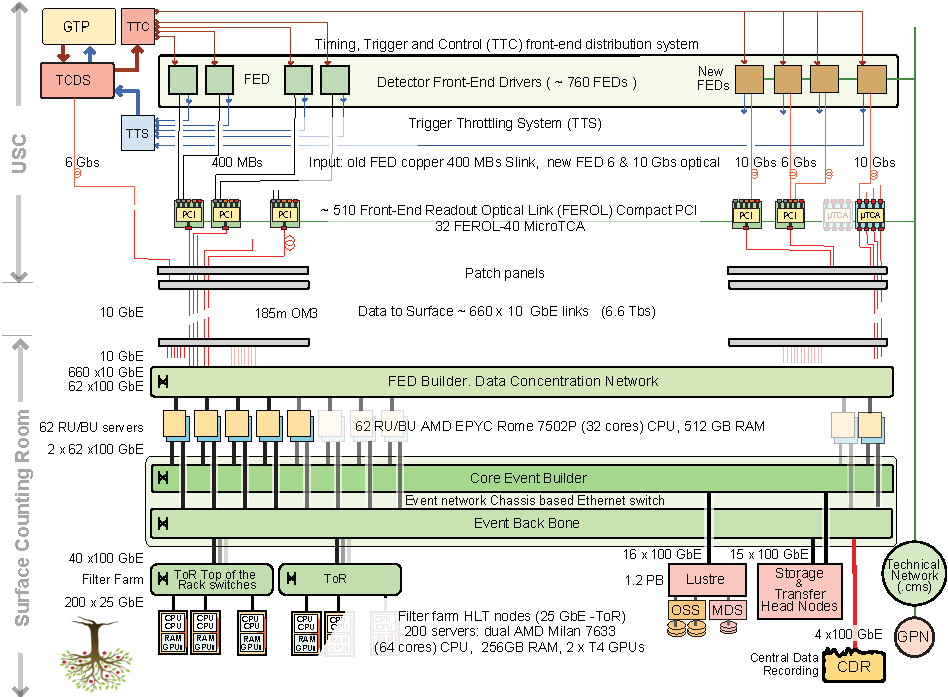
\includegraphics[width=0.7\textwidth]{figures/DAQRun3.pdf}
  \caption{Diagram of the Run 3 DAQ system.}
   \label{fig:DAQ3}
\end{figure}

The output data are then sent back to the BUs, where they are further merged and their management is handed over to the storage and transfer system (STS).
The STS  transfer the data to a (Lustre-based) cluster file system, whence they are finally sent to their final destination:
Tier-0,
DQM
or the calibration cluster.
The DAQ3 was also designed with two characteristics that the demonstrator should respect: 
i) it is \emph{pipelined}, so the data should follow an unidirectional flow;
ii) it is \emph{democratic}, in the sense that all elements (RUs, BUs, FUs) are treated equally.

%%% Thiago testing the GitHub integration
% I want to work at the LHC!
% I want to work at the FCC!

\subsection{Conceptual DAQ Design for Phase-2}

\subsection{System Feasibility: Preliminary Calculation}

As the overarching goal of the NGT project is to reconstruct and save all the L1-accepted data, 
our first assumption is that the system will have to buffer all the data of a run whilst 
running the optimal calibrations.
The size of the data buffer $B$ can be estimated by the following formula
\begin{equation}
B = A^{\text{L1}} \times \tau \times E \times s
\label{eq:buffersize}
\end{equation}
where $A^{\text{L1}}$ is the Level-1 trigger accept rate,
$\tau$ is the period during which we have to buffer the data,
$E$ is the event size and
$s$ is a safety factor.
For a first calculation, we take the Run 4 estimates from the DAQ-HLT TDR:
-- $L1A$ = 500\kHz, $E$ = 6.1\,MB --
and assume a flat 50\% safety factor ($s$ = 1.5).
The discussion on the magnitude of the buffer period $\tau$ is more subtle and will be done in the next section.

\subsubsection{Buffer Period}

The amount of time during which the data has to be buffered depends on many factors,
and we add a set of working hypotheses to be able to estimate its value.
\begin{itemize}
\item The buffer period has to be longer than the amount of time needed to derive the calibrations.
A relevant timescale is the PCL completion time, which we know from experience to take close to eight hours.
We know from experience that the PCL takes, in average, 8 hours to run for completion.
Some of the longest runs, however, may need additional time; a long run from LHC fill 10200 took data during more than 13 hours
(delivering close to $900\pbinv$), and
the PCL took more than 10 hours to finish,
as seen in Fig.~\ref{fig:fill10200PCL}.
Notice that, in offline reconstruction, Tier-0 starts the PCL only after the run end; 
therefore the 48 hours limit for the start of prompt reconstruction applies to 
the sum of run duration and the PCL duration.
After the calibration is done the data has to be buffered for some more time in order to allow the NGT reconstruction to run.
Therefore, we choose to use a representative value of \emph{12 hours}.
\begin{figure}[htbp]
   \centering
	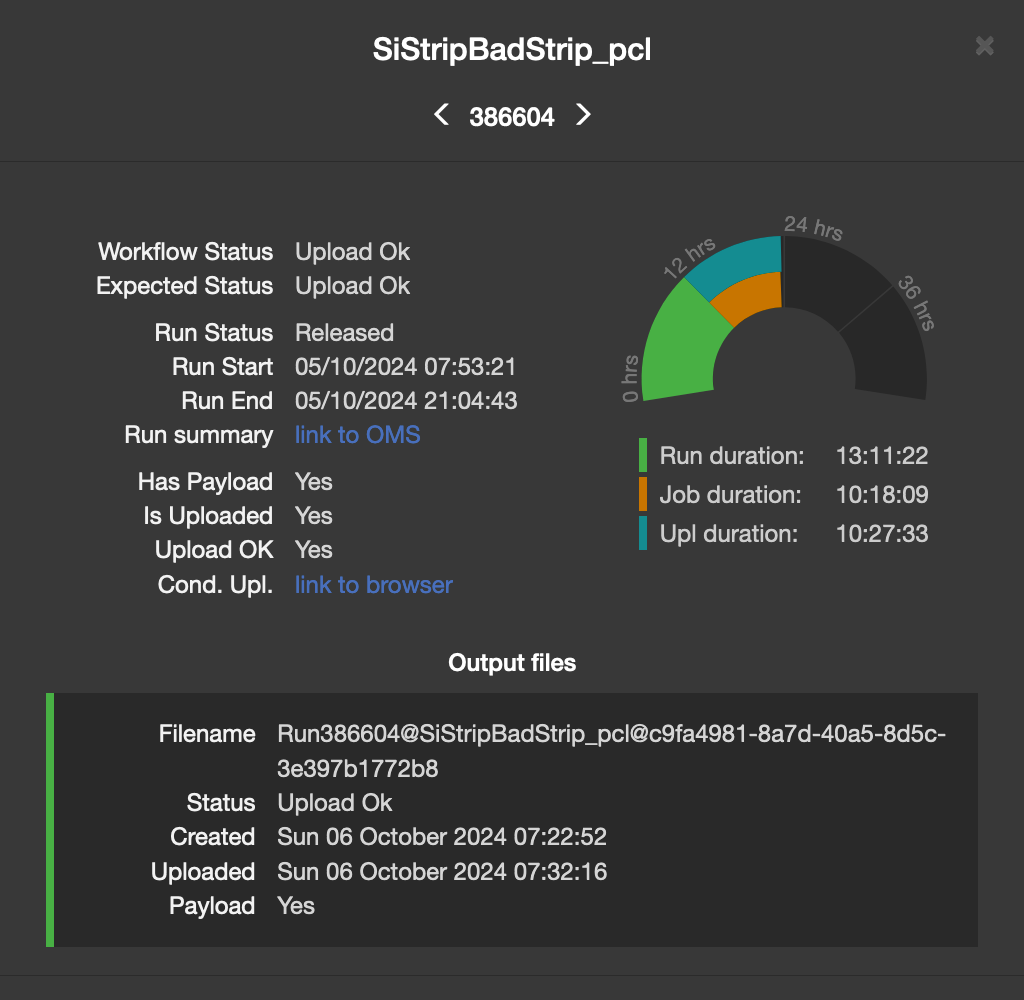
\includegraphics[width=0.7\textwidth]{figures/fill10200PCL.png}
   \caption{PCL monitoring of the silicon strip bad components calibration for a run of LHC fill 10200 (the number 386604 refers to internal CMS bookkeeping).
   The run took data over more than 13 hours, whilst the PCL ran for over 10 hours.}
   \label{fig:fill10200PCL}
\end{figure}
\item On the other hand, the buffer has to be large enough to store all the data from an LHC fill, as per our first assumption,
but that calculation has to take into account the LHC duty cycle, so we use the following working hypotheses:
\begin{itemize}
\item The High-Luminosity LHC will work in a $\sim70\%$ duty cycle, meaning that in a 24-hour period there will be 17 hours of stable beams and 7 hours of interfill (including injection and ramp).
\item Levelling will once again be used to keep the effective luminosity at a given level.
Following the Run 3 historic performance, we assume that the 17 hours of stable beams will be divided into 10 hours of levelling and 7 hours of lumi decay phase.
\item Again following the Run 3 performance, we assume that the luminosity (as well as the pileup) in the decay phase will average out to $\sim80\%$ of levelled luminosity.
\item We assume that the event size $E$ scales linearly with pileup.
\item We assume that the Level-1 accept rate $L1A$ will be kept constant even during the decay phase. 
\item The 7 hours of downtime are effectively free from the point of view of data buffering for NGT.
\end{itemize}
\end{itemize}

By simply substituting $\tau$ = 12 hours in Eq.~\ref{eq:buffersize}, we arrive at a buffer size $B$ = 200 PB.
The second calculation that accounts for the LHC duty cycle amounts to three applications of the same equation,
and is summarised in Table~\ref{tab:bufferWithDutyCycle}. In that case, we arrive at a buffer size of $B$ = 258 PB for a 24 hour period.
Noting that the two results agree within $\sim25\%$, and that many more assumptions go into the second calculation, for the purposes of this report we proceed with the \textbf{200\,PB} figure.
% Requires the booktabs if the memoir class is not being used
\begin{table}[htbp]
   \centering
   %\topcaption{Table captions are better up top} % requires the topcapt package
   \begin{tabular}{@{} lrrrrr @{}} % Column formatting, @{} suppresses leading/trailing space
      \toprule
		Phase & Duration (h) & $A^{\text{L1}}$ (kHz) & $E$ (MB) & Safety factor & Buffer (PB)\\
      	\midrule
		Levelling & 10 & 500 & 6.1 & 1.5 & 165 \\
		Decay     &  7 & 500 & 4.9 & 1.5 &  93 \\
		Interfill &  7 &  -- &  -- &  -- &   0 \\
		\midrule
\textbf{Total}    & \textbf{24} & N/A & N/A & N/A & \textbf{258}\\ 
      \bottomrule
   \end{tabular}
   \caption{Calculation for NGT buffer size accounting for LHC duty cycle. 
   This modelling concludes that a 258\,PB buffer is adequate for a 24-hour period.}
   \label{tab:bufferWithDutyCycle}
\end{table}

We can compare the proposed NGT buffer size to a number of similar systems.
The current storage capacity of the CMS Run 3 DAQ system is 1.2\,PB.
The LHCb experiment implemented a similar dataflow in their DAQ system, 
with events accepted by their HLT1 system held in a 30\,PB buffer,
used for real-time alignment and calibration,
and finally passed on to their HLT2 system.
\textcolor{red}{Lastly, the CMS Tier-0 holds a disk buffer of 11\,PB for incoming raw data from Point 5 to be held on for prompt reconstruction,
as well as a disk buffer of 25\,PB for reconstructed data before it is transferred to other sites in the WLCG.}
We also note that experience from the LHCb system shows that the reading/writing speed of the disks decreases when they fill up,
which justifies the consideration of a large safety factor ($s = 1.5$).

\subsubsection{Nodes for the Optimal Calibration}

The computer nodes for the optimal calibration have to be integrated in the DAQ system.
The alignment and calibration algorithms need built events to run over, so these nodes need to be downstream of the BUs.

\subsubsection{Additional Output from NGT Workflow}




